
% Default to the notebook output style



% Tell the templating engine what output template we want to use.

% Default to the notebook output style


% Inherit from the specified cell style.




    
\documentclass{article}

    
    
    \usepackage{graphicx} % Used to insert images
    \usepackage{adjustbox} % Used to constrain images to a maximum size 
    \usepackage{color} % Allow colors to be defined
    \usepackage{enumerate} % Needed for markdown enumerations to work
    \usepackage{geometry} % Used to adjust the document margins
    \usepackage{amsmath} % Equations
    \usepackage{amssymb} % Equations
    \usepackage{eurosym} % defines \euro
    \usepackage[mathletters]{ucs} % Extended unicode (utf-8) support
    \usepackage[utf8x]{inputenc} % Allow utf-8 characters in the tex document
    \usepackage{fancyvrb} % verbatim replacement that allows latex
    \usepackage{grffile} % extends the file name processing of package graphics 
                         % to support a larger range 
    % The hyperref package gives us a pdf with properly built
    % internal navigation ('pdf bookmarks' for the table of contents,
    % internal cross-reference links, web links for URLs, etc.)
    \usepackage{hyperref}
    \usepackage{longtable} % longtable support required by pandoc >1.10
    \usepackage{booktabs}  % table support for pandoc > 1.12.2
    

    
    
    \definecolor{orange}{cmyk}{0,0.4,0.8,0.2}
    \definecolor{darkorange}{rgb}{.71,0.21,0.01}
    \definecolor{darkgreen}{rgb}{.12,.54,.11}
    \definecolor{myteal}{rgb}{.26, .44, .56}
    \definecolor{gray}{gray}{0.45}
    \definecolor{lightgray}{gray}{.95}
    \definecolor{mediumgray}{gray}{.8}
    \definecolor{inputbackground}{rgb}{.95, .95, .85}
    \definecolor{outputbackground}{rgb}{.95, .95, .95}
    \definecolor{traceback}{rgb}{1, .95, .95}
    % ansi colors
    \definecolor{red}{rgb}{.6,0,0}
    \definecolor{green}{rgb}{0,.65,0}
    \definecolor{brown}{rgb}{0.6,0.6,0}
    \definecolor{blue}{rgb}{0,.145,.698}
    \definecolor{purple}{rgb}{.698,.145,.698}
    \definecolor{cyan}{rgb}{0,.698,.698}
    \definecolor{lightgray}{gray}{0.5}
    
    % bright ansi colors
    \definecolor{darkgray}{gray}{0.25}
    \definecolor{lightred}{rgb}{1.0,0.39,0.28}
    \definecolor{lightgreen}{rgb}{0.48,0.99,0.0}
    \definecolor{lightblue}{rgb}{0.53,0.81,0.92}
    \definecolor{lightpurple}{rgb}{0.87,0.63,0.87}
    \definecolor{lightcyan}{rgb}{0.5,1.0,0.83}
    
    % commands and environments needed by pandoc snippets
    % extracted from the output of `pandoc -s`
    \providecommand{\tightlist}{%
      \setlength{\itemsep}{0pt}\setlength{\parskip}{0pt}}
    \DefineVerbatimEnvironment{Highlighting}{Verbatim}{commandchars=\\\{\}}
    % Add ',fontsize=\small' for more characters per line
    \newenvironment{Shaded}{}{}
    \newcommand{\KeywordTok}[1]{\textcolor[rgb]{0.00,0.44,0.13}{\textbf{{#1}}}}
    \newcommand{\DataTypeTok}[1]{\textcolor[rgb]{0.56,0.13,0.00}{{#1}}}
    \newcommand{\DecValTok}[1]{\textcolor[rgb]{0.25,0.63,0.44}{{#1}}}
    \newcommand{\BaseNTok}[1]{\textcolor[rgb]{0.25,0.63,0.44}{{#1}}}
    \newcommand{\FloatTok}[1]{\textcolor[rgb]{0.25,0.63,0.44}{{#1}}}
    \newcommand{\CharTok}[1]{\textcolor[rgb]{0.25,0.44,0.63}{{#1}}}
    \newcommand{\StringTok}[1]{\textcolor[rgb]{0.25,0.44,0.63}{{#1}}}
    \newcommand{\CommentTok}[1]{\textcolor[rgb]{0.38,0.63,0.69}{\textit{{#1}}}}
    \newcommand{\OtherTok}[1]{\textcolor[rgb]{0.00,0.44,0.13}{{#1}}}
    \newcommand{\AlertTok}[1]{\textcolor[rgb]{1.00,0.00,0.00}{\textbf{{#1}}}}
    \newcommand{\FunctionTok}[1]{\textcolor[rgb]{0.02,0.16,0.49}{{#1}}}
    \newcommand{\RegionMarkerTok}[1]{{#1}}
    \newcommand{\ErrorTok}[1]{\textcolor[rgb]{1.00,0.00,0.00}{\textbf{{#1}}}}
    \newcommand{\NormalTok}[1]{{#1}}
    
    % Define a nice break command that doesn't care if a line doesn't already
    % exist.
    \def\br{\hspace*{\fill} \\* }
    % Math Jax compatability definitions
    \def\gt{>}
    \def\lt{<}
    % Document parameters
    \title{three\_compartment\_model}
    
    
    

    % Pygments definitions
    
\makeatletter
\def\PY@reset{\let\PY@it=\relax \let\PY@bf=\relax%
    \let\PY@ul=\relax \let\PY@tc=\relax%
    \let\PY@bc=\relax \let\PY@ff=\relax}
\def\PY@tok#1{\csname PY@tok@#1\endcsname}
\def\PY@toks#1+{\ifx\relax#1\empty\else%
    \PY@tok{#1}\expandafter\PY@toks\fi}
\def\PY@do#1{\PY@bc{\PY@tc{\PY@ul{%
    \PY@it{\PY@bf{\PY@ff{#1}}}}}}}
\def\PY#1#2{\PY@reset\PY@toks#1+\relax+\PY@do{#2}}

\expandafter\def\csname PY@tok@gd\endcsname{\def\PY@tc##1{\textcolor[rgb]{0.63,0.00,0.00}{##1}}}
\expandafter\def\csname PY@tok@gu\endcsname{\let\PY@bf=\textbf\def\PY@tc##1{\textcolor[rgb]{0.50,0.00,0.50}{##1}}}
\expandafter\def\csname PY@tok@gt\endcsname{\def\PY@tc##1{\textcolor[rgb]{0.00,0.27,0.87}{##1}}}
\expandafter\def\csname PY@tok@gs\endcsname{\let\PY@bf=\textbf}
\expandafter\def\csname PY@tok@gr\endcsname{\def\PY@tc##1{\textcolor[rgb]{1.00,0.00,0.00}{##1}}}
\expandafter\def\csname PY@tok@cm\endcsname{\let\PY@it=\textit\def\PY@tc##1{\textcolor[rgb]{0.25,0.50,0.50}{##1}}}
\expandafter\def\csname PY@tok@vg\endcsname{\def\PY@tc##1{\textcolor[rgb]{0.10,0.09,0.49}{##1}}}
\expandafter\def\csname PY@tok@m\endcsname{\def\PY@tc##1{\textcolor[rgb]{0.40,0.40,0.40}{##1}}}
\expandafter\def\csname PY@tok@mh\endcsname{\def\PY@tc##1{\textcolor[rgb]{0.40,0.40,0.40}{##1}}}
\expandafter\def\csname PY@tok@go\endcsname{\def\PY@tc##1{\textcolor[rgb]{0.53,0.53,0.53}{##1}}}
\expandafter\def\csname PY@tok@ge\endcsname{\let\PY@it=\textit}
\expandafter\def\csname PY@tok@vc\endcsname{\def\PY@tc##1{\textcolor[rgb]{0.10,0.09,0.49}{##1}}}
\expandafter\def\csname PY@tok@il\endcsname{\def\PY@tc##1{\textcolor[rgb]{0.40,0.40,0.40}{##1}}}
\expandafter\def\csname PY@tok@cs\endcsname{\let\PY@it=\textit\def\PY@tc##1{\textcolor[rgb]{0.25,0.50,0.50}{##1}}}
\expandafter\def\csname PY@tok@cp\endcsname{\def\PY@tc##1{\textcolor[rgb]{0.74,0.48,0.00}{##1}}}
\expandafter\def\csname PY@tok@gi\endcsname{\def\PY@tc##1{\textcolor[rgb]{0.00,0.63,0.00}{##1}}}
\expandafter\def\csname PY@tok@gh\endcsname{\let\PY@bf=\textbf\def\PY@tc##1{\textcolor[rgb]{0.00,0.00,0.50}{##1}}}
\expandafter\def\csname PY@tok@ni\endcsname{\let\PY@bf=\textbf\def\PY@tc##1{\textcolor[rgb]{0.60,0.60,0.60}{##1}}}
\expandafter\def\csname PY@tok@nl\endcsname{\def\PY@tc##1{\textcolor[rgb]{0.63,0.63,0.00}{##1}}}
\expandafter\def\csname PY@tok@nn\endcsname{\let\PY@bf=\textbf\def\PY@tc##1{\textcolor[rgb]{0.00,0.00,1.00}{##1}}}
\expandafter\def\csname PY@tok@no\endcsname{\def\PY@tc##1{\textcolor[rgb]{0.53,0.00,0.00}{##1}}}
\expandafter\def\csname PY@tok@na\endcsname{\def\PY@tc##1{\textcolor[rgb]{0.49,0.56,0.16}{##1}}}
\expandafter\def\csname PY@tok@nb\endcsname{\def\PY@tc##1{\textcolor[rgb]{0.00,0.50,0.00}{##1}}}
\expandafter\def\csname PY@tok@nc\endcsname{\let\PY@bf=\textbf\def\PY@tc##1{\textcolor[rgb]{0.00,0.00,1.00}{##1}}}
\expandafter\def\csname PY@tok@nd\endcsname{\def\PY@tc##1{\textcolor[rgb]{0.67,0.13,1.00}{##1}}}
\expandafter\def\csname PY@tok@ne\endcsname{\let\PY@bf=\textbf\def\PY@tc##1{\textcolor[rgb]{0.82,0.25,0.23}{##1}}}
\expandafter\def\csname PY@tok@nf\endcsname{\def\PY@tc##1{\textcolor[rgb]{0.00,0.00,1.00}{##1}}}
\expandafter\def\csname PY@tok@si\endcsname{\let\PY@bf=\textbf\def\PY@tc##1{\textcolor[rgb]{0.73,0.40,0.53}{##1}}}
\expandafter\def\csname PY@tok@s2\endcsname{\def\PY@tc##1{\textcolor[rgb]{0.73,0.13,0.13}{##1}}}
\expandafter\def\csname PY@tok@vi\endcsname{\def\PY@tc##1{\textcolor[rgb]{0.10,0.09,0.49}{##1}}}
\expandafter\def\csname PY@tok@nt\endcsname{\let\PY@bf=\textbf\def\PY@tc##1{\textcolor[rgb]{0.00,0.50,0.00}{##1}}}
\expandafter\def\csname PY@tok@nv\endcsname{\def\PY@tc##1{\textcolor[rgb]{0.10,0.09,0.49}{##1}}}
\expandafter\def\csname PY@tok@s1\endcsname{\def\PY@tc##1{\textcolor[rgb]{0.73,0.13,0.13}{##1}}}
\expandafter\def\csname PY@tok@kd\endcsname{\let\PY@bf=\textbf\def\PY@tc##1{\textcolor[rgb]{0.00,0.50,0.00}{##1}}}
\expandafter\def\csname PY@tok@sh\endcsname{\def\PY@tc##1{\textcolor[rgb]{0.73,0.13,0.13}{##1}}}
\expandafter\def\csname PY@tok@sc\endcsname{\def\PY@tc##1{\textcolor[rgb]{0.73,0.13,0.13}{##1}}}
\expandafter\def\csname PY@tok@sx\endcsname{\def\PY@tc##1{\textcolor[rgb]{0.00,0.50,0.00}{##1}}}
\expandafter\def\csname PY@tok@bp\endcsname{\def\PY@tc##1{\textcolor[rgb]{0.00,0.50,0.00}{##1}}}
\expandafter\def\csname PY@tok@c1\endcsname{\let\PY@it=\textit\def\PY@tc##1{\textcolor[rgb]{0.25,0.50,0.50}{##1}}}
\expandafter\def\csname PY@tok@kc\endcsname{\let\PY@bf=\textbf\def\PY@tc##1{\textcolor[rgb]{0.00,0.50,0.00}{##1}}}
\expandafter\def\csname PY@tok@c\endcsname{\let\PY@it=\textit\def\PY@tc##1{\textcolor[rgb]{0.25,0.50,0.50}{##1}}}
\expandafter\def\csname PY@tok@mf\endcsname{\def\PY@tc##1{\textcolor[rgb]{0.40,0.40,0.40}{##1}}}
\expandafter\def\csname PY@tok@err\endcsname{\def\PY@bc##1{\setlength{\fboxsep}{0pt}\fcolorbox[rgb]{1.00,0.00,0.00}{1,1,1}{\strut ##1}}}
\expandafter\def\csname PY@tok@mb\endcsname{\def\PY@tc##1{\textcolor[rgb]{0.40,0.40,0.40}{##1}}}
\expandafter\def\csname PY@tok@ss\endcsname{\def\PY@tc##1{\textcolor[rgb]{0.10,0.09,0.49}{##1}}}
\expandafter\def\csname PY@tok@sr\endcsname{\def\PY@tc##1{\textcolor[rgb]{0.73,0.40,0.53}{##1}}}
\expandafter\def\csname PY@tok@mo\endcsname{\def\PY@tc##1{\textcolor[rgb]{0.40,0.40,0.40}{##1}}}
\expandafter\def\csname PY@tok@kn\endcsname{\let\PY@bf=\textbf\def\PY@tc##1{\textcolor[rgb]{0.00,0.50,0.00}{##1}}}
\expandafter\def\csname PY@tok@mi\endcsname{\def\PY@tc##1{\textcolor[rgb]{0.40,0.40,0.40}{##1}}}
\expandafter\def\csname PY@tok@gp\endcsname{\let\PY@bf=\textbf\def\PY@tc##1{\textcolor[rgb]{0.00,0.00,0.50}{##1}}}
\expandafter\def\csname PY@tok@o\endcsname{\def\PY@tc##1{\textcolor[rgb]{0.40,0.40,0.40}{##1}}}
\expandafter\def\csname PY@tok@kr\endcsname{\let\PY@bf=\textbf\def\PY@tc##1{\textcolor[rgb]{0.00,0.50,0.00}{##1}}}
\expandafter\def\csname PY@tok@s\endcsname{\def\PY@tc##1{\textcolor[rgb]{0.73,0.13,0.13}{##1}}}
\expandafter\def\csname PY@tok@kp\endcsname{\def\PY@tc##1{\textcolor[rgb]{0.00,0.50,0.00}{##1}}}
\expandafter\def\csname PY@tok@w\endcsname{\def\PY@tc##1{\textcolor[rgb]{0.73,0.73,0.73}{##1}}}
\expandafter\def\csname PY@tok@kt\endcsname{\def\PY@tc##1{\textcolor[rgb]{0.69,0.00,0.25}{##1}}}
\expandafter\def\csname PY@tok@ow\endcsname{\let\PY@bf=\textbf\def\PY@tc##1{\textcolor[rgb]{0.67,0.13,1.00}{##1}}}
\expandafter\def\csname PY@tok@sb\endcsname{\def\PY@tc##1{\textcolor[rgb]{0.73,0.13,0.13}{##1}}}
\expandafter\def\csname PY@tok@k\endcsname{\let\PY@bf=\textbf\def\PY@tc##1{\textcolor[rgb]{0.00,0.50,0.00}{##1}}}
\expandafter\def\csname PY@tok@se\endcsname{\let\PY@bf=\textbf\def\PY@tc##1{\textcolor[rgb]{0.73,0.40,0.13}{##1}}}
\expandafter\def\csname PY@tok@sd\endcsname{\let\PY@it=\textit\def\PY@tc##1{\textcolor[rgb]{0.73,0.13,0.13}{##1}}}

\def\PYZbs{\char`\\}
\def\PYZus{\char`\_}
\def\PYZob{\char`\{}
\def\PYZcb{\char`\}}
\def\PYZca{\char`\^}
\def\PYZam{\char`\&}
\def\PYZlt{\char`\<}
\def\PYZgt{\char`\>}
\def\PYZsh{\char`\#}
\def\PYZpc{\char`\%}
\def\PYZdl{\char`\$}
\def\PYZhy{\char`\-}
\def\PYZsq{\char`\'}
\def\PYZdq{\char`\"}
\def\PYZti{\char`\~}
% for compatibility with earlier versions
\def\PYZat{@}
\def\PYZlb{[}
\def\PYZrb{]}
\makeatother


    % Exact colors from NB
    \definecolor{incolor}{rgb}{0.0, 0.0, 0.5}
    \definecolor{outcolor}{rgb}{0.545, 0.0, 0.0}



    
    % Prevent overflowing lines due to hard-to-break entities
    \sloppy 
    % Setup hyperref package
    \hypersetup{
      breaklinks=true,  % so long urls are correctly broken across lines
      colorlinks=true,
      urlcolor=blue,
      linkcolor=darkorange,
      citecolor=darkgreen,
      }
    % Slightly bigger margins than the latex defaults
    
    \geometry{verbose,tmargin=1in,bmargin=1in,lmargin=1in,rmargin=1in}
    
    

    \begin{document}
    
    
    \author{Joanna Lewis and Peter White}\title{A model for chlamydia surveillance data}

\date{\today}
\maketitle

    
    

    
    \section{A model for chlamydia surveillance
data}\label{a-model-for-chlamydia-surveillance-data}

We propose a three-compartment model of chlamydia infection, testing and
screening in a closed population, as illustrated below. Uninfected
individuals (U) become infected with a constant incidence, and move to
either the asymptomatic-infected (A) or symptomatic-infected (S) pool.
Asymptomatic-infected individuals may leave A and return to U by
spontaneous clearance of their infection or by detection and treatment
under a screening programme. Symptomatic individuals too may clear their
infection spontaneously or be screened, but will also seek treatment at
a rate which is typically much higher than the rates of spontaneous
clearance or screening.

    \begin{footnotesize}
        \begin{Verbatim}[commandchars=\\\{\}]
{\color{incolor}In [{\color{incolor}1}]:} \PY{k+kn}{from} \PY{n+nn}{IPython.display} \PY{k+kn}{import} \PY{n}{Image}
        \PY{n}{Image}\PY{p}{(}\PY{n}{filename}\PY{o}{=}\PY{l+s}{\PYZdq{}}\PY{l+s}{figures/3\PYZus{}comp.png}\PY{l+s}{\PYZdq{}}\PY{p}{,} \PY{n}{width}\PY{o}{=}\PY{l+m+mi}{500}\PY{p}{)}
\end{Verbatim}
    \end{footnotesize}
\begin{footnotesize}
		\texttt{\color{outcolor}Out[{\color{outcolor}1}]:}\texttt{\color{outcolor}Out[{\color{outcolor}1}]:}
    
    \begin{figure}
        \begin{center}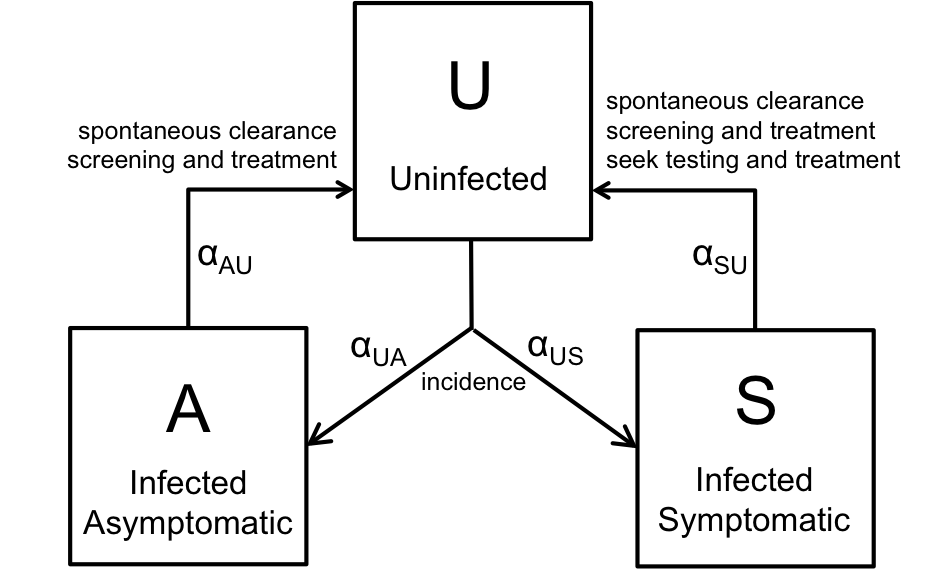
\includegraphics[width=10cm]{three_compartment_model_files/three_compartment_model_1_0.png}\end{center}
        \caption{A model of chlamydia infection, clearance, testing and treatment.}
        \label{fig:model}
    \end{figure}
    

	\end{footnotesize}
    This dynamic model has a steady-state solution which depends on the
transition rates \(\alpha_{UA}\), \(\alpha_{AU}\), \(\alpha_{US}\) and
\(\alpha_{SU}\):

    \begin{footnotesize}
        \begin{Verbatim}[commandchars=\\\{\}]
{\color{incolor}In [{\color{incolor}2}]:} \PY{k+kn}{import} \PY{n+nn}{sympy} \PY{k+kn}{as} \PY{n+nn}{sym}
        \PY{k+kn}{from} \PY{n+nn}{sympy} \PY{k+kn}{import} \PY{o}{*}
        \PY{n}{A}\PY{p}{,} \PY{n}{U}\PY{p}{,} \PY{n}{S} \PY{o}{=} \PY{n}{symbols}\PY{p}{(}\PY{l+s}{\PYZdq{}}\PY{l+s}{A U S}\PY{l+s}{\PYZdq{}}\PY{p}{)}
        \PY{n}{alpha\PYZus{}UA}\PY{p}{,} \PY{n}{alpha\PYZus{}AU}\PY{p}{,} \PY{n}{alpha\PYZus{}US}\PY{p}{,} \PY{n}{alpha\PYZus{}SU}  \PY{o}{=} \PY{n}{symbols}\PY{p}{(}\PY{l+s}{\PYZdq{}}\PY{l+s}{alpha\PYZus{}UA alpha\PYZus{}AU alpha\PYZus{}US alpha\PYZus{}SU}\PY{l+s}{\PYZdq{}}\PY{p}{)}
        
        \PY{n}{model\PYZus{}dyn} \PY{o}{=} \PY{p}{[}
            \PY{n}{alpha\PYZus{}UA}\PY{o}{*}\PY{n}{U} \PY{o}{\PYZhy{}} \PY{n}{alpha\PYZus{}AU}\PY{o}{*}\PY{n}{A}\PY{p}{,}
            \PY{n}{alpha\PYZus{}AU}\PY{o}{*}\PY{n}{A} \PY{o}{+} \PY{n}{alpha\PYZus{}SU}\PY{o}{*}\PY{n}{S} \PY{o}{\PYZhy{}} \PY{p}{(}\PY{n}{alpha\PYZus{}UA} \PY{o}{+} \PY{n}{alpha\PYZus{}US}\PY{p}{)}\PY{o}{*}\PY{n}{U}\PY{p}{,}
            \PY{n}{alpha\PYZus{}US}\PY{o}{*}\PY{n}{U} \PY{o}{\PYZhy{}} \PY{n}{alpha\PYZus{}SU}\PY{o}{*}\PY{n}{S}\PY{p}{,}
            \PY{n}{A} \PY{o}{+} \PY{n}{U} \PY{o}{+} \PY{n}{S} \PY{o}{\PYZhy{}} \PY{l+m+mi}{1} \PY{c}{\PYZsh{} this equation sets the total population size to 1}
            \PY{p}{]}
        
        \PY{c}{\PYZsh{} steady\PYZhy{}state solution}
        \PY{n}{sol\PYZus{}dyn} \PY{o}{=} \PY{n}{solve}\PY{p}{(}\PY{n}{model\PYZus{}dyn}\PY{p}{,} \PY{n}{A}\PY{p}{,} \PY{n}{U}\PY{p}{,} \PY{n}{S}\PY{p}{)}
        
        \PY{c}{\PYZsh{} functions for calculating the proportion of the population in each compartment at }
        \PY{c}{\PYZsh{} steady state, given transition rates between compartments}
        \PY{n}{dyn\PYZus{}fun} \PY{o}{=} \PY{n}{lambdify}\PY{p}{(}\PY{p}{(}\PY{n}{alpha\PYZus{}UA}\PY{p}{,} \PY{n}{alpha\PYZus{}AU}\PY{p}{,} \PY{n}{alpha\PYZus{}US}\PY{p}{,} \PY{n}{alpha\PYZus{}SU}\PY{p}{)}\PY{p}{,} \PY{n}{sol\PYZus{}dyn}\PY{p}{[}\PY{n}{A}\PY{p}{]} \PY{o}{+} \PY{n}{sol\PYZus{}dyn}\PY{p}{[}\PY{n}{S}\PY{p}{]}\PY{p}{)}
        \PY{n}{U\PYZus{}fun} \PY{o}{=} \PY{n}{lambdify}\PY{p}{(}\PY{p}{(}\PY{n}{alpha\PYZus{}UA}\PY{p}{,} \PY{n}{alpha\PYZus{}AU}\PY{p}{,} \PY{n}{alpha\PYZus{}US}\PY{p}{,} \PY{n}{alpha\PYZus{}SU}\PY{p}{)}\PY{p}{,} \PY{n}{sol\PYZus{}dyn}\PY{p}{[}\PY{n}{U}\PY{p}{]}\PY{p}{)}
        \PY{n}{A\PYZus{}fun} \PY{o}{=} \PY{n}{lambdify}\PY{p}{(}\PY{p}{(}\PY{n}{alpha\PYZus{}UA}\PY{p}{,} \PY{n}{alpha\PYZus{}AU}\PY{p}{,} \PY{n}{alpha\PYZus{}US}\PY{p}{,} \PY{n}{alpha\PYZus{}SU}\PY{p}{)}\PY{p}{,} \PY{n}{sol\PYZus{}dyn}\PY{p}{[}\PY{n}{A}\PY{p}{]}\PY{p}{)}
        \PY{n}{S\PYZus{}fun} \PY{o}{=} \PY{n}{lambdify}\PY{p}{(}\PY{p}{(}\PY{n}{alpha\PYZus{}UA}\PY{p}{,} \PY{n}{alpha\PYZus{}AU}\PY{p}{,} \PY{n}{alpha\PYZus{}US}\PY{p}{,} \PY{n}{alpha\PYZus{}SU}\PY{p}{)}\PY{p}{,} \PY{n}{sol\PYZus{}dyn}\PY{p}{[}\PY{n}{S}\PY{p}{]}\PY{p}{)}
        
        \PY{n}{sol\PYZus{}dyn}
\end{Verbatim}
    \end{footnotesize}

    \begin{footnotesize}
            \begin{Verbatim}[commandchars=\\\{\}]
{\color{outcolor}Out[{\color{outcolor}2}]:} \{S: alpha\_AU*alpha\_US/(alpha\_AU*alpha\_US + alpha\_SU*(alpha\_AU + alpha\_UA)),
         U: alpha\_AU*alpha\_SU/(alpha\_AU*alpha\_US + alpha\_SU*(alpha\_AU + alpha\_UA)),
         A: alpha\_SU*alpha\_UA/(alpha\_AU*alpha\_US + alpha\_SU*(alpha\_AU + alpha\_UA))\}
\end{Verbatim}
    \end{footnotesize}
        
    The transition rates are functions of parameters describing behaviour
and the natural history of infection:

\[
\begin{align}
\alpha_{UA} &= \mbox{incidence} \times (1 - p_{symptomatic}) \\
\alpha_{AU} &= \mbox{rate of spontaneous clearance} + \mbox{rate of screening} \times p_{true positive} \\
\alpha_{US} &= \mbox{incidence} \times p_{symptomatic} \\
\alpha_{SU} &= \mbox{rate of spontaneous clearance} + \mbox{rate of screening} \times p_{true positive} + \mbox{rate of symptomatic testing} \times p_{true positive}
\end{align}
\]

Assuming all tests conducted are included in the surveillance data, the
number of tests reported per unit time will be:

\[
\mbox{rate of testing} = \mbox{rate of screening} + S \times \mbox{rate of symptomatic testing}
\]

And the number of diagnoses per unit time will be:

\begin{multline*}
\mbox{rate of new diagnoses} = (A+S) \times (\mbox{rate of screening} \times p_{true positive}) \\
+ (U \times \mbox{rate of screening} \times p_{false positive}) \\
+ (S \times \mbox{rate of symptomatic testing} \times p_{truepositive})
\end{multline*}

Let's assume that:

\begin{itemize}
\tightlist
\item
  51.0\% of incident infections are asymptomatic.
\item
  Infections (whether symptomatic or not) clear spontaneously or through
  background antibiotic use at a rate 0.396 per year.
\item
  Symptomatic cases seek and obtain testing and treatment at a rate 14.2
  per year.
\item
  97.1\% of tests in infected individuals return a positive result.
\item
  0.314\% of tests in uninfected individuals return a positive result.
\end{itemize}

    \begin{footnotesize}
        \begin{Verbatim}[commandchars=\\\{\}]
{\color{incolor}In [{\color{incolor}3}]:} \PY{n}{p\PYZus{}asymp} \PY{o}{=} \PY{l+m+mf}{0.510}
        \PY{n}{sc} \PY{o}{=} \PY{l+m+mf}{0.396}
        \PY{n}{att\PYZus{}symp} \PY{o}{=} \PY{l+m+mf}{14.2}
        \PY{n}{p\PYZus{}true\PYZus{}pos} \PY{o}{=} \PY{l+m+mf}{0.971}
        \PY{n}{p\PYZus{}false\PYZus{}pos} \PY{o}{=} \PY{l+m+mf}{0.00314}
\end{Verbatim}
    \end{footnotesize}

    It is then possible to calculate the steady-state proportion of the
population in each compartment given the rate of screening and
incidence, and from these proportions to calculate the total prevalence,
and the rates of new tests and diagnoses.

    \begin{footnotesize}
        \begin{Verbatim}[commandchars=\\\{\}]
{\color{incolor}In [{\color{incolor}4}]:} \PY{o}{\PYZpc{}}\PY{k}{matplotlib} inline
        \PY{k+kn}{from} \PY{n+nn}{numpy} \PY{k+kn}{import} \PY{o}{*}
        \PY{k+kn}{import} \PY{n+nn}{matplotlib.pyplot} \PY{k+kn}{as} \PY{n+nn}{plt}
        
        \PY{n}{inc} \PY{o}{=} \PY{n}{linspace}\PY{p}{(}\PY{l+m+mi}{0}\PY{p}{,} \PY{l+m+mf}{0.5}\PY{p}{,} \PY{l+m+mi}{101}\PY{p}{)} \PY{c}{\PYZsh{} incidence}
        \PY{n}{scr} \PY{o}{=} \PY{n}{linspace}\PY{p}{(}\PY{l+m+mi}{0}\PY{p}{,} \PY{l+m+mf}{0.5}\PY{p}{,} \PY{l+m+mi}{101}\PY{p}{)} \PY{c}{\PYZsh{} screening}
        \PY{n}{inc}\PY{p}{,}\PY{n}{scr} \PY{o}{=} \PY{n}{meshgrid}\PY{p}{(}\PY{n}{inc}\PY{p}{,} \PY{n}{scr}\PY{p}{)}
        
        \PY{c}{\PYZsh{} proportion of population in each compartment}
        \PY{n}{ZU} \PY{o}{=} \PY{n}{U\PYZus{}fun}\PY{p}{(}\PY{n}{inc}\PY{o}{*}\PY{n}{p\PYZus{}asymp}\PY{p}{,} \PY{n}{sc} \PY{o}{+} \PY{n}{scr}\PY{o}{*}\PY{n}{p\PYZus{}true\PYZus{}pos}\PY{p}{,} \PY{n}{inc}\PY{o}{*}\PY{p}{(}\PY{l+m+mi}{1}\PY{o}{\PYZhy{}}\PY{n}{p\PYZus{}asymp}\PY{p}{)}\PY{p}{,} \PY{n}{sc} \PY{o}{+} \PY{n}{scr}\PY{o}{*}\PY{n}{p\PYZus{}true\PYZus{}pos} \PY{o}{+} \PY{n}{att\PYZus{}symp}\PY{o}{*}\PY{n}{p\PYZus{}true\PYZus{}pos}\PY{p}{)}
        \PY{n}{ZA} \PY{o}{=} \PY{n}{A\PYZus{}fun}\PY{p}{(}\PY{n}{inc}\PY{o}{*}\PY{n}{p\PYZus{}asymp}\PY{p}{,} \PY{n}{sc} \PY{o}{+} \PY{n}{scr}\PY{o}{*}\PY{n}{p\PYZus{}true\PYZus{}pos}\PY{p}{,} \PY{n}{inc}\PY{o}{*}\PY{p}{(}\PY{l+m+mi}{1}\PY{o}{\PYZhy{}}\PY{n}{p\PYZus{}asymp}\PY{p}{)}\PY{p}{,} \PY{n}{sc} \PY{o}{+} \PY{n}{scr}\PY{o}{*}\PY{n}{p\PYZus{}true\PYZus{}pos} \PY{o}{+} \PY{n}{att\PYZus{}symp}\PY{o}{*}\PY{n}{p\PYZus{}true\PYZus{}pos}\PY{p}{)}
        \PY{n}{ZS} \PY{o}{=} \PY{n}{S\PYZus{}fun}\PY{p}{(}\PY{n}{inc}\PY{o}{*}\PY{n}{p\PYZus{}asymp}\PY{p}{,} \PY{n}{sc} \PY{o}{+} \PY{n}{scr}\PY{o}{*}\PY{n}{p\PYZus{}true\PYZus{}pos}\PY{p}{,} \PY{n}{inc}\PY{o}{*}\PY{p}{(}\PY{l+m+mi}{1}\PY{o}{\PYZhy{}}\PY{n}{p\PYZus{}asymp}\PY{p}{)}\PY{p}{,} \PY{n}{sc} \PY{o}{+} \PY{n}{scr}\PY{o}{*}\PY{n}{p\PYZus{}true\PYZus{}pos} \PY{o}{+} \PY{n}{att\PYZus{}symp}\PY{o}{*}\PY{n}{p\PYZus{}true\PYZus{}pos}\PY{p}{)}
        
        \PY{n}{Zprev} \PY{o}{=} \PY{l+m+mi}{1} \PY{o}{\PYZhy{}} \PY{n}{ZU}
        \PY{n}{Ztest} \PY{o}{=} \PY{n}{scr} \PY{o}{+} \PY{n}{ZS}\PY{o}{*}\PY{n}{att\PYZus{}symp}
        \PY{n}{Zdiag} \PY{o}{=} \PY{p}{(}\PY{n}{ZA}\PY{o}{+}\PY{n}{ZS}\PY{p}{)}\PY{o}{*}\PY{n}{scr}\PY{o}{*}\PY{n}{p\PYZus{}true\PYZus{}pos} \PY{o}{+} \PY{n}{ZU}\PY{o}{*}\PY{n}{scr}\PY{o}{*}\PY{n}{p\PYZus{}false\PYZus{}pos} \PY{o}{+} \PY{n}{ZS}\PY{o}{*}\PY{n}{att\PYZus{}symp}\PY{o}{*}\PY{n}{p\PYZus{}true\PYZus{}pos}
\end{Verbatim}
    \end{footnotesize}

    \begin{footnotesize}
        \begin{Verbatim}[commandchars=\\\{\}]
{\color{incolor}In [{\color{incolor}5}]:} \PY{n}{fig} \PY{o}{=} \PY{n}{plt}\PY{o}{.}\PY{n}{figure}\PY{p}{(}\PY{n}{figsize} \PY{o}{=} \PY{p}{(}\PY{l+m+mi}{12}\PY{p}{,} \PY{l+m+mi}{7}\PY{p}{)}\PY{p}{)}
        
        \PY{n}{ax1} \PY{o}{=} \PY{n}{fig}\PY{o}{.}\PY{n}{add\PYZus{}subplot}\PY{p}{(}\PY{l+m+mi}{231}\PY{p}{)}
        \PY{n}{p} \PY{o}{=} \PY{n}{ax1}\PY{o}{.}\PY{n}{pcolor}\PY{p}{(}\PY{n}{inc}\PY{p}{,}\PY{n}{scr}\PY{p}{,} \PY{n}{ZU}\PY{p}{)}
        \PY{n}{cb} \PY{o}{=} \PY{n}{fig}\PY{o}{.}\PY{n}{colorbar}\PY{p}{(}\PY{n}{p}\PY{p}{,} \PY{n}{ax}\PY{o}{=}\PY{n}{ax1}\PY{p}{)}
        \PY{c}{\PYZsh{}ax1.set\PYZus{}xlabel(\PYZsq{}Incidence\PYZsq{})}
        \PY{n}{ax1}\PY{o}{.}\PY{n}{set\PYZus{}ylabel}\PY{p}{(}\PY{l+s}{\PYZsq{}}\PY{l+s}{Screening Rate}\PY{l+s}{\PYZsq{}}\PY{p}{)}
        \PY{n}{t} \PY{o}{=} \PY{n}{ax1}\PY{o}{.}\PY{n}{text}\PY{p}{(}\PY{l+m+mf}{0.25}\PY{p}{,} \PY{l+m+mf}{0.45}\PY{p}{,} \PY{l+s}{\PYZsq{}}\PY{l+s}{Uninfected}\PY{l+s}{\PYZsq{}}\PY{p}{,} \PY{n}{ha}\PY{o}{=}\PY{l+s}{\PYZsq{}}\PY{l+s}{center}\PY{l+s}{\PYZsq{}}\PY{p}{,} \PY{n}{size}\PY{o}{=}\PY{l+s}{\PYZsq{}}\PY{l+s}{large}\PY{l+s}{\PYZsq{}}\PY{p}{)}
        \PY{n}{t}\PY{o}{.}\PY{n}{set\PYZus{}bbox}\PY{p}{(}\PY{n+nb}{dict}\PY{p}{(}\PY{n}{facecolor}\PY{o}{=}\PY{l+s}{\PYZsq{}}\PY{l+s}{white}\PY{l+s}{\PYZsq{}}\PY{p}{,} \PY{n}{alpha}\PY{o}{=}\PY{l+m+mf}{0.7}\PY{p}{,} \PY{n}{edgecolor}\PY{o}{=}\PY{l+s}{\PYZsq{}}\PY{l+s}{None}\PY{l+s}{\PYZsq{}}\PY{p}{)}\PY{p}{)}
        \PY{n}{ax1}\PY{o}{.}\PY{n}{set\PYZus{}ylim}\PY{p}{(}\PY{l+m+mi}{0}\PY{p}{,} \PY{l+m+mf}{0.5}\PY{p}{)}
        \PY{n}{ax1}\PY{o}{.}\PY{n}{set\PYZus{}xlim}\PY{p}{(}\PY{l+m+mi}{0}\PY{p}{,} \PY{l+m+mf}{0.5}\PY{p}{)}
        
        \PY{n}{ax2} \PY{o}{=} \PY{n}{fig}\PY{o}{.}\PY{n}{add\PYZus{}subplot}\PY{p}{(}\PY{l+m+mi}{232}\PY{p}{)}
        \PY{n}{p} \PY{o}{=} \PY{n}{ax2}\PY{o}{.}\PY{n}{pcolor}\PY{p}{(}\PY{n}{inc}\PY{p}{,}\PY{n}{scr}\PY{p}{,} \PY{n}{ZS}\PY{p}{)}
        \PY{n}{cb} \PY{o}{=} \PY{n}{fig}\PY{o}{.}\PY{n}{colorbar}\PY{p}{(}\PY{n}{p}\PY{p}{,} \PY{n}{ax}\PY{o}{=}\PY{n}{ax2}\PY{p}{)}
        \PY{n}{t} \PY{o}{=} \PY{n}{ax2}\PY{o}{.}\PY{n}{text}\PY{p}{(}\PY{l+m+mf}{0.25}\PY{p}{,} \PY{l+m+mf}{0.45}\PY{p}{,} \PY{l+s}{\PYZsq{}}\PY{l+s}{Infected, Symptomatic}\PY{l+s}{\PYZsq{}}\PY{p}{,} \PY{n}{ha}\PY{o}{=}\PY{l+s}{\PYZsq{}}\PY{l+s}{center}\PY{l+s}{\PYZsq{}}\PY{p}{,} \PY{n}{size}\PY{o}{=}\PY{l+s}{\PYZsq{}}\PY{l+s}{large}\PY{l+s}{\PYZsq{}}\PY{p}{)}
        \PY{n}{t}\PY{o}{.}\PY{n}{set\PYZus{}bbox}\PY{p}{(}\PY{n+nb}{dict}\PY{p}{(}\PY{n}{facecolor}\PY{o}{=}\PY{l+s}{\PYZsq{}}\PY{l+s}{white}\PY{l+s}{\PYZsq{}}\PY{p}{,} \PY{n}{alpha}\PY{o}{=}\PY{l+m+mf}{0.7}\PY{p}{,} \PY{n}{edgecolor}\PY{o}{=}\PY{l+s}{\PYZsq{}}\PY{l+s}{None}\PY{l+s}{\PYZsq{}}\PY{p}{)}\PY{p}{)}
        \PY{n}{ax2}\PY{o}{.}\PY{n}{set\PYZus{}ylim}\PY{p}{(}\PY{l+m+mi}{0}\PY{p}{,} \PY{l+m+mf}{0.5}\PY{p}{)}
        \PY{n}{ax2}\PY{o}{.}\PY{n}{set\PYZus{}xlim}\PY{p}{(}\PY{l+m+mi}{0}\PY{p}{,} \PY{l+m+mf}{0.5}\PY{p}{)}
        
        \PY{n}{ax3} \PY{o}{=} \PY{n}{fig}\PY{o}{.}\PY{n}{add\PYZus{}subplot}\PY{p}{(}\PY{l+m+mi}{233}\PY{p}{)}
        \PY{n}{p} \PY{o}{=} \PY{n}{ax3}\PY{o}{.}\PY{n}{pcolor}\PY{p}{(}\PY{n}{inc}\PY{p}{,}\PY{n}{scr}\PY{p}{,} \PY{n}{ZA}\PY{p}{)}
        \PY{n}{cb} \PY{o}{=} \PY{n}{fig}\PY{o}{.}\PY{n}{colorbar}\PY{p}{(}\PY{n}{p}\PY{p}{,} \PY{n}{ax}\PY{o}{=}\PY{n}{ax3}\PY{p}{)}
        \PY{n}{t} \PY{o}{=} \PY{n}{ax3}\PY{o}{.}\PY{n}{text}\PY{p}{(}\PY{l+m+mf}{0.25}\PY{p}{,} \PY{l+m+mf}{0.45}\PY{p}{,} \PY{l+s}{\PYZsq{}}\PY{l+s}{Infected, Asymptomatic}\PY{l+s}{\PYZsq{}}\PY{p}{,} \PY{n}{ha}\PY{o}{=}\PY{l+s}{\PYZsq{}}\PY{l+s}{center}\PY{l+s}{\PYZsq{}}\PY{p}{,} \PY{n}{size}\PY{o}{=}\PY{l+s}{\PYZsq{}}\PY{l+s}{large}\PY{l+s}{\PYZsq{}}\PY{p}{)}
        \PY{n}{t}\PY{o}{.}\PY{n}{set\PYZus{}bbox}\PY{p}{(}\PY{n+nb}{dict}\PY{p}{(}\PY{n}{facecolor}\PY{o}{=}\PY{l+s}{\PYZsq{}}\PY{l+s}{white}\PY{l+s}{\PYZsq{}}\PY{p}{,} \PY{n}{alpha}\PY{o}{=}\PY{l+m+mf}{0.7}\PY{p}{,} \PY{n}{edgecolor}\PY{o}{=}\PY{l+s}{\PYZsq{}}\PY{l+s}{None}\PY{l+s}{\PYZsq{}}\PY{p}{)}\PY{p}{)}
        \PY{n}{ax3}\PY{o}{.}\PY{n}{set\PYZus{}ylim}\PY{p}{(}\PY{l+m+mi}{0}\PY{p}{,} \PY{l+m+mf}{0.5}\PY{p}{)}
        \PY{n}{ax3}\PY{o}{.}\PY{n}{set\PYZus{}xlim}\PY{p}{(}\PY{l+m+mi}{0}\PY{p}{,} \PY{l+m+mf}{0.5}\PY{p}{)}
        
        \PY{n}{ax4} \PY{o}{=} \PY{n}{fig}\PY{o}{.}\PY{n}{add\PYZus{}subplot}\PY{p}{(}\PY{l+m+mi}{234}\PY{p}{)}
        \PY{n}{p} \PY{o}{=} \PY{n}{ax4}\PY{o}{.}\PY{n}{pcolor}\PY{p}{(}\PY{n}{inc}\PY{p}{,}\PY{n}{scr}\PY{p}{,} \PY{n}{Zprev}\PY{p}{)}
        \PY{n}{cb} \PY{o}{=} \PY{n}{fig}\PY{o}{.}\PY{n}{colorbar}\PY{p}{(}\PY{n}{p}\PY{p}{,} \PY{n}{ax}\PY{o}{=}\PY{n}{ax4}\PY{p}{)}
        \PY{n}{ax4}\PY{o}{.}\PY{n}{set\PYZus{}xlabel}\PY{p}{(}\PY{l+s}{\PYZsq{}}\PY{l+s}{Incidence}\PY{l+s}{\PYZsq{}}\PY{p}{)}
        \PY{n}{ax4}\PY{o}{.}\PY{n}{set\PYZus{}ylabel}\PY{p}{(}\PY{l+s}{\PYZsq{}}\PY{l+s}{Screening Rate}\PY{l+s}{\PYZsq{}}\PY{p}{)}
        \PY{n}{t} \PY{o}{=} \PY{n}{ax4}\PY{o}{.}\PY{n}{text}\PY{p}{(}\PY{l+m+mf}{0.25}\PY{p}{,} \PY{l+m+mf}{0.45}\PY{p}{,} \PY{l+s}{\PYZsq{}}\PY{l+s}{Prevalence}\PY{l+s}{\PYZsq{}}\PY{p}{,} \PY{n}{ha}\PY{o}{=}\PY{l+s}{\PYZsq{}}\PY{l+s}{center}\PY{l+s}{\PYZsq{}}\PY{p}{,} \PY{n}{size}\PY{o}{=}\PY{l+s}{\PYZsq{}}\PY{l+s}{large}\PY{l+s}{\PYZsq{}}\PY{p}{)}
        \PY{n}{t}\PY{o}{.}\PY{n}{set\PYZus{}bbox}\PY{p}{(}\PY{n+nb}{dict}\PY{p}{(}\PY{n}{facecolor}\PY{o}{=}\PY{l+s}{\PYZsq{}}\PY{l+s}{white}\PY{l+s}{\PYZsq{}}\PY{p}{,} \PY{n}{alpha}\PY{o}{=}\PY{l+m+mf}{0.7}\PY{p}{,} \PY{n}{edgecolor}\PY{o}{=}\PY{l+s}{\PYZsq{}}\PY{l+s}{None}\PY{l+s}{\PYZsq{}}\PY{p}{)}\PY{p}{)}
        \PY{n}{ax4}\PY{o}{.}\PY{n}{set\PYZus{}ylim}\PY{p}{(}\PY{l+m+mi}{0}\PY{p}{,} \PY{l+m+mf}{0.5}\PY{p}{)}
        \PY{n}{ax4}\PY{o}{.}\PY{n}{set\PYZus{}xlim}\PY{p}{(}\PY{l+m+mi}{0}\PY{p}{,} \PY{l+m+mf}{0.5}\PY{p}{)}
        
        \PY{n}{ax5} \PY{o}{=} \PY{n}{fig}\PY{o}{.}\PY{n}{add\PYZus{}subplot}\PY{p}{(}\PY{l+m+mi}{235}\PY{p}{)}
        \PY{n}{p} \PY{o}{=} \PY{n}{ax5}\PY{o}{.}\PY{n}{pcolor}\PY{p}{(}\PY{n}{inc}\PY{p}{,}\PY{n}{scr}\PY{p}{,} \PY{n}{Ztest}\PY{p}{)}
        \PY{n}{cb} \PY{o}{=} \PY{n}{fig}\PY{o}{.}\PY{n}{colorbar}\PY{p}{(}\PY{n}{p}\PY{p}{,} \PY{n}{ax}\PY{o}{=}\PY{n}{ax5}\PY{p}{)}
        \PY{n}{ax5}\PY{o}{.}\PY{n}{set\PYZus{}xlabel}\PY{p}{(}\PY{l+s}{\PYZsq{}}\PY{l+s}{Incidence}\PY{l+s}{\PYZsq{}}\PY{p}{)}
        \PY{n}{t} \PY{o}{=} \PY{n}{ax5}\PY{o}{.}\PY{n}{text}\PY{p}{(}\PY{l+m+mf}{0.25}\PY{p}{,} \PY{l+m+mf}{0.45}\PY{p}{,} \PY{l+s}{\PYZsq{}}\PY{l+s}{Testing Rate}\PY{l+s}{\PYZsq{}}\PY{p}{,} \PY{n}{ha}\PY{o}{=}\PY{l+s}{\PYZsq{}}\PY{l+s}{center}\PY{l+s}{\PYZsq{}}\PY{p}{,} \PY{n}{size}\PY{o}{=}\PY{l+s}{\PYZsq{}}\PY{l+s}{large}\PY{l+s}{\PYZsq{}}\PY{p}{)}
        \PY{n}{t}\PY{o}{.}\PY{n}{set\PYZus{}bbox}\PY{p}{(}\PY{n+nb}{dict}\PY{p}{(}\PY{n}{facecolor}\PY{o}{=}\PY{l+s}{\PYZsq{}}\PY{l+s}{white}\PY{l+s}{\PYZsq{}}\PY{p}{,} \PY{n}{alpha}\PY{o}{=}\PY{l+m+mf}{0.7}\PY{p}{,} \PY{n}{edgecolor}\PY{o}{=}\PY{l+s}{\PYZsq{}}\PY{l+s}{None}\PY{l+s}{\PYZsq{}}\PY{p}{)}\PY{p}{)}
        \PY{n}{ax5}\PY{o}{.}\PY{n}{set\PYZus{}ylim}\PY{p}{(}\PY{l+m+mi}{0}\PY{p}{,} \PY{l+m+mf}{0.5}\PY{p}{)}
        \PY{n}{ax5}\PY{o}{.}\PY{n}{set\PYZus{}xlim}\PY{p}{(}\PY{l+m+mi}{0}\PY{p}{,} \PY{l+m+mf}{0.5}\PY{p}{)}
        
        \PY{n}{ax6} \PY{o}{=} \PY{n}{fig}\PY{o}{.}\PY{n}{add\PYZus{}subplot}\PY{p}{(}\PY{l+m+mi}{236}\PY{p}{)}
        \PY{n}{p} \PY{o}{=} \PY{n}{ax6}\PY{o}{.}\PY{n}{pcolor}\PY{p}{(}\PY{n}{inc}\PY{p}{,}\PY{n}{scr}\PY{p}{,} \PY{n}{Zdiag}\PY{p}{)}
        \PY{n}{cb} \PY{o}{=} \PY{n}{fig}\PY{o}{.}\PY{n}{colorbar}\PY{p}{(}\PY{n}{p}\PY{p}{,} \PY{n}{ax}\PY{o}{=}\PY{n}{ax6}\PY{p}{)}
        \PY{n}{ax6}\PY{o}{.}\PY{n}{set\PYZus{}xlabel}\PY{p}{(}\PY{l+s}{\PYZsq{}}\PY{l+s}{Incidence}\PY{l+s}{\PYZsq{}}\PY{p}{)}
        \PY{n}{t} \PY{o}{=} \PY{n}{ax6}\PY{o}{.}\PY{n}{text}\PY{p}{(}\PY{l+m+mf}{0.25}\PY{p}{,} \PY{l+m+mf}{0.45}\PY{p}{,} \PY{l+s}{\PYZsq{}}\PY{l+s}{Diagnosis Rate}\PY{l+s}{\PYZsq{}}\PY{p}{,} \PY{n}{ha}\PY{o}{=}\PY{l+s}{\PYZsq{}}\PY{l+s}{center}\PY{l+s}{\PYZsq{}}\PY{p}{,} \PY{n}{size}\PY{o}{=}\PY{l+s}{\PYZsq{}}\PY{l+s}{large}\PY{l+s}{\PYZsq{}}\PY{p}{)}
        \PY{n}{t}\PY{o}{.}\PY{n}{set\PYZus{}bbox}\PY{p}{(}\PY{n+nb}{dict}\PY{p}{(}\PY{n}{facecolor}\PY{o}{=}\PY{l+s}{\PYZsq{}}\PY{l+s}{white}\PY{l+s}{\PYZsq{}}\PY{p}{,} \PY{n}{alpha}\PY{o}{=}\PY{l+m+mf}{0.7}\PY{p}{,} \PY{n}{edgecolor}\PY{o}{=}\PY{l+s}{\PYZsq{}}\PY{l+s}{None}\PY{l+s}{\PYZsq{}}\PY{p}{)}\PY{p}{)}
        \PY{n}{ax6}\PY{o}{.}\PY{n}{set\PYZus{}ylim}\PY{p}{(}\PY{l+m+mi}{0}\PY{p}{,} \PY{l+m+mf}{0.5}\PY{p}{)}
        \PY{n}{ax6}\PY{o}{.}\PY{n}{set\PYZus{}xlim}\PY{p}{(}\PY{l+m+mi}{0}\PY{p}{,} \PY{l+m+mf}{0.5}\PY{p}{)}
        
        \PY{n}{plt}\PY{o}{.}\PY{n}{show}\PY{p}{(}\PY{p}{)}   
\end{Verbatim}
    \end{footnotesize}

    \begin{figure}
        \begin{center}\adjustimage{max size={0.9\linewidth}{0.4\paperheight}}{three_compartment_model_files/three_compartment_model_8_0.png}\end{center}
        \caption{Upper row: the effects of incidence and screening rate on the proportion of individuals who are uninfected, infected-symptomatic and infected-asymptomatic in the model at steady state. Lower row: prevalence, testing and diagnosis rates corresponding to each combination of incidence and screening rate.}
        \label{fig:model}
    \end{figure}
    
    From the figures, it is clear that a particular pair of observed testing
and diagnosis rates corresponds to a single point in the (incidence,
screening rate) plane, which in turn corresponds to a particular
prevalence. Note, however, that this mapping depends on the parameter
values which have been assumed.


    % Add a bibliography block to the postdoc
    
    
    
    \end{document}
